% CVPR/ICCV: two-column teaser at the top of page 1 (kit's strip method)
\begin{strip}
\centering
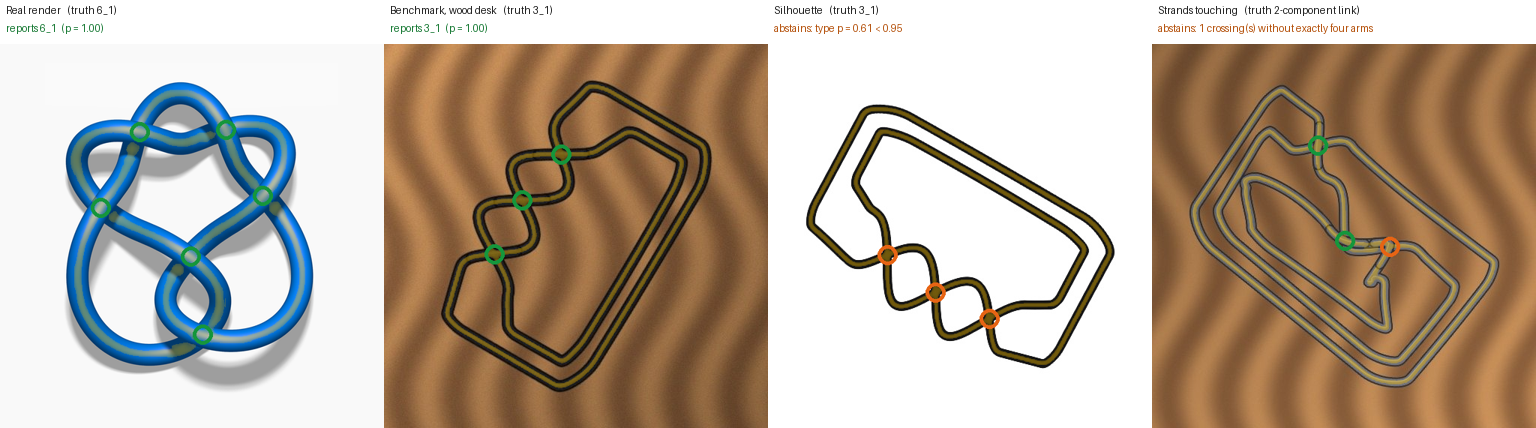
\includegraphics[width=\linewidth]{../figures/teaser.png}
\captionsetup{hypcap=false}
\captionof{figure}{\textbf{Read the diagram, compute the knot, abstain when the image is not
enough.} Green circles: crossings read with \ou{} probability $>0.9$; yellow: the
predicted strand centre-line. A real render and a benchmark cable are identified
exactly. On a silhouette the \ou{} reading disagrees across test-time views, so the
type probability stays below 0.95 and the system abstains. Where two strands touch, a
crossing loses an arm and the system abstains rather than guess.}
\captionsetup{hypcap=true}
\label{fig:teaser}
\end{strip}
